\chapter{Connected transversals of 5-colorings}
By Theorem \ref{thm:5}, all graphs on five vertices and, at most, six edges have (*) properties. 
We will show the properties that a counter-example must satisfy for a graph with five vertices and at least seven edges to fail to have property (*).

\begin{lemma}
 Let $H$ be a graph on five vertices, Let $G$ be a graph with coloring $\mathcal{C}$ and transversal $T$ such that $H$ is isomorphic to $H(G, \mathcal{C}, T)$;
 if $H$ is not a rooted minor of $G$, then $G$ is 2-connected.
\end{lemma}

\begin{proof}
 Let $G$ be the minimal such graph, the minimality of $G$ implies that $(\forall A, B \in \mathcal{C}: A \neq B)$ $G[A \cup B]$ is a single path between the transversal vertices of corresponding colors from $T$.

 Assume that $G$ is 1-connected for contradiction. Then, a cut vertex exists in $G$; let us denote it as $x$. 
    
 We have six cases to consider.
 In the following figure, the black vertices are the transversal vertices $T$ on which we cannot build a rooted minor isomorphic to $H$, and if 
 a vertex is with a hole, then it is a non-transversal vertex.
       
    \begin{figure}[h]
       \centering
       \vspace{0.3cm}
       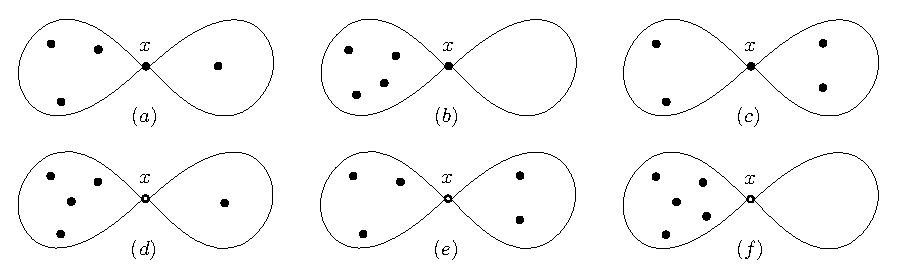
\includegraphics[width=13cm]{img/hourglass+1-cases.eps}
       \vspace{0.3cm}
       \caption{All cases of cut vertices in a 1-connected graph}
       \label{fig:2connected_counterexamples}
   \end{figure}
   
 Notice that for the cases (a), (b), and (c), the cut vertex $x$ is a transversal vertex.
   

   $H$ does not have a vertex of degree one, otherwise By Theorem \ref{thm:6}, we have that $K_4$ has property
 (*) and $K_4 + 1$ vertex with degree one also has property (*) (By Theorem \ref{thm:2}), and since property (*) is inhereted to the subgraphs of 
 the graph (By Theorem \ref{thm:1}), then $H$ would have property (*), which is a contradiction.

 We have that all vertices in $H$ have degrees at least two, and if all of them are exactly two, then $H$ is a cycle, and By Theorem 4 in \cite{matthias_2022}, we have that
 all cycles have property (*), hence $H$ would have property (*), which is a contradiction.

 So we have that $H$ has at least one vertex of degree at least three; if it is exactly three and the rest are two, then by handshake lemma, we have at least 
 two vertices of degree three. If its' degree is four and the rest of the vertices have degree two, then we get that the graph $H$ is 
 the hourglass graph, which by Theorem \ref{thm:5} has property (*), hence $H$ would have property (*), which is a contradiction. So we have
 at least two vertices in $H$ that have a degree of at least three, and the rest have a degree of at least two.

 Let $R$ be the subgraph of the right side of the cut and $L$ be the subgraph of the left side of the cut.
 
 \begin{itemize}
    \item \textbf{Case (a)}: 
    Let us denote the transversal vertex in $R$ as $y$, and since 
 all vertices in $H$ have degrees at least two, then we have to have at least two Kempe chains between $y$ and two other transversal vertices in $G$. All paths from $y$ to other transversal vertices may only pass through
    $x$ because except $x$, all other transversals are in $L$; since $x$ is a transversal vertex itself, we can have a kempe chain from $y$ to $x$, but since $y$ and $x$ have different
 colors, we cannot have more Kempe chains going from $y$ through $x$ to other transversal vertices. Hence, we have only one Kempe chain from $y$ to other transversal vertices, bringing us to a contradiction.


    \item \textbf{Case (b)}: 
    Unlike case (a), we can realize all necessary Kempe chains. If no Kempe chain between transversals has edges in $R$, we can contract
 all vertices of $R$ into $x$ and preserve all Kempe chains between transversals; hence, $G$ was not a minimal graph, a contradiction.
 So let us assume there is some Kempe chain which has a subpath in $R$; since all Kempe chains start from $L$, such a Kempe chain has to pass through $x$; this means that if 
    $G$ is a counter-example; after contracting all edges of the $R$ into $x$, we still have left Kempe chains between all necessary transversals in $L$, but we got a smaller graph
 which still should be a counter-example; if the contracted version is not a counter-example, then it would mean $G$ was not a counter-example in the beginning since we could get a 
 rooted minor $H$ from G. Hence, the graph $G$ is not minimal, which is a contradiction.

    \item \textbf{Case (c)}: 
    If both vertices with degrees at least three are in $R$, let us denote them as $y, z$, then we can only have Kempe chains from $y$
 to $x$ and $z$, and from $z$ to $x$ and $y$, but $deg(y) >= 3, deg(z) >= 3$ in $H$, which is a contradiction since they can have 
 at most two Kempe chains in $G$ in this case. Then, assume only one vertex of degree, at least three, is in $R$, and let it be $y$. Similarly, we get that $y$ can have
 at most two Kempe chains, which is a contradiction. Symmetrically, the same holds if $x$ and $y$ were in $L$ or one of them was in $L$; hence, in all cases, we get a contradiction.

    \item \textbf{Case (d)}: 
    The vertex in $R$ has a degree of at least two. Hence, the color of $x$ is the color of the vertex itself,
so we can contract the paths from it to $x$ and still get the counter-example, which is a contradiction since the graph $G$ was not minimal.
    \item \textbf{Case (e)}:
    Let vertices in $L$ be denoted as $a,b,c$ and the vertices in $R$ as $y, z$, if we have at least one vertex with degree at least three in $R$, let it be $y$, then we can have
one Kempe chain between $y$ and $z$, and at least two Kempe chains from $y$ to $L$, hence $x$ has the color of $y$, but now since $z$ has 
degree at least two, at least one Kempe chain from $z$ should go to $L$, and it can pass only through $x$, since the color of $x$ is the same color as $y$, the 
Kempe chain from $z$, even if it includes $x$, can only be connected to $y$; hence, it cannot pass to $L$, which is a contradiction.
So we have that both vertices with degrees at least three are in $L$; in $L$ we have three vertices, and if all of them are maximally connected to each other, 
we get the $abc$ cycle, and since two vertices in $L$ have a degree of at least three, at least two Kempe chains should pass from $L$ to $R$, both of them pass through $x$, 
so both of them should be connected to the same transversal vertex in $R$, WLOG it is $y$, but then $z$ in $R$ can only be connected to $y$ if it has
Kempe chain to any other transversal than $y$, it has to pass through $x$ but $x$ has color of $y$, so the only Kempe chain from $z$ including $x$ can go to $y$
which is a contradiction since in $H$ $deg(z) >= 2$, we only can have one Kempe chain in $G$ from $z$
    \item \textbf{Case (f)}:
    We could contract all the vertices from $R$ into $x$ and still get the counter-example
    because all the Kempe chains still exist between the transversals, it contradicts the minimality of $G$.
 \end{itemize}
Thus, $G$ is 2-connected.
\end{proof}